\documentclass[10pt,a4paper]{article}
\usepackage[T1]{fontenc}
\usepackage[a4paper]{geometry}
\usepackage{xcolor}
\usepackage{amssymb}
\usepackage{amsmath}
\usepackage{graphicx}
\usepackage{tabularx}
\usepackage{multirow}
\usepackage{subfigure}
\usepackage{verbatim}
\usepackage{fancyhdr}
\usepackage{listings}
\usepackage{../common/espacs}

%\input{../common/commands.tex}

\title{Exercise Session 4}
\date{October 26, 2012}

\pagestyle{fancy}
\headheight 35pt

\rhead{\copyright~2006/2012}

\newcommand{\vv}[1]{\mathbf{#1}}

\begin{document}
\lstset{language=[ISO]C++}
\maketitle

\section*{Google PageRank}

Dalla sua nascita, Google ha impiegato brevissimo tempo per imporsi
come il pi\`u utilizzato motore di ricerca rispetto a tutti i
concorrenti. Il successo \`e dipeso dalla accuratezza delle risposte,
molto superiore a quelle di altri motori di ricerca.
Google infatti stila una propria classifica (\emph{ranking})
dell'importanza delle pagine web, per ordinare i risultati proposti;
molto spesso questa classifica \`e proprio quella desiderata l'utente.

L'algoritmo che ordina le pagine web per importanza \`e denominato
\emph{PageRank} ed \`e stato sviluppato da S.~Brin e L.~Page presso
la Stanford University \cite{Brin1998}.
Il principio su cui si basa \`e il seguente:
\begin{itemize}

    \item se una pagina web A ha un collegamento (\emph{link}) verso una
        pagina B, questo \`e interpretato come un voto di A in favore di B
        (cio\`e alza B in graduatoria);

    \item i votanti non sono tutti uguali: il voto di chi \`e alto in
        classifica (cio\`e ha ricevuto molti link) vale maggiormente di quello di chi \`e
        in basso.

\end{itemize}

\begin{figure}[htbp]
    \centering
    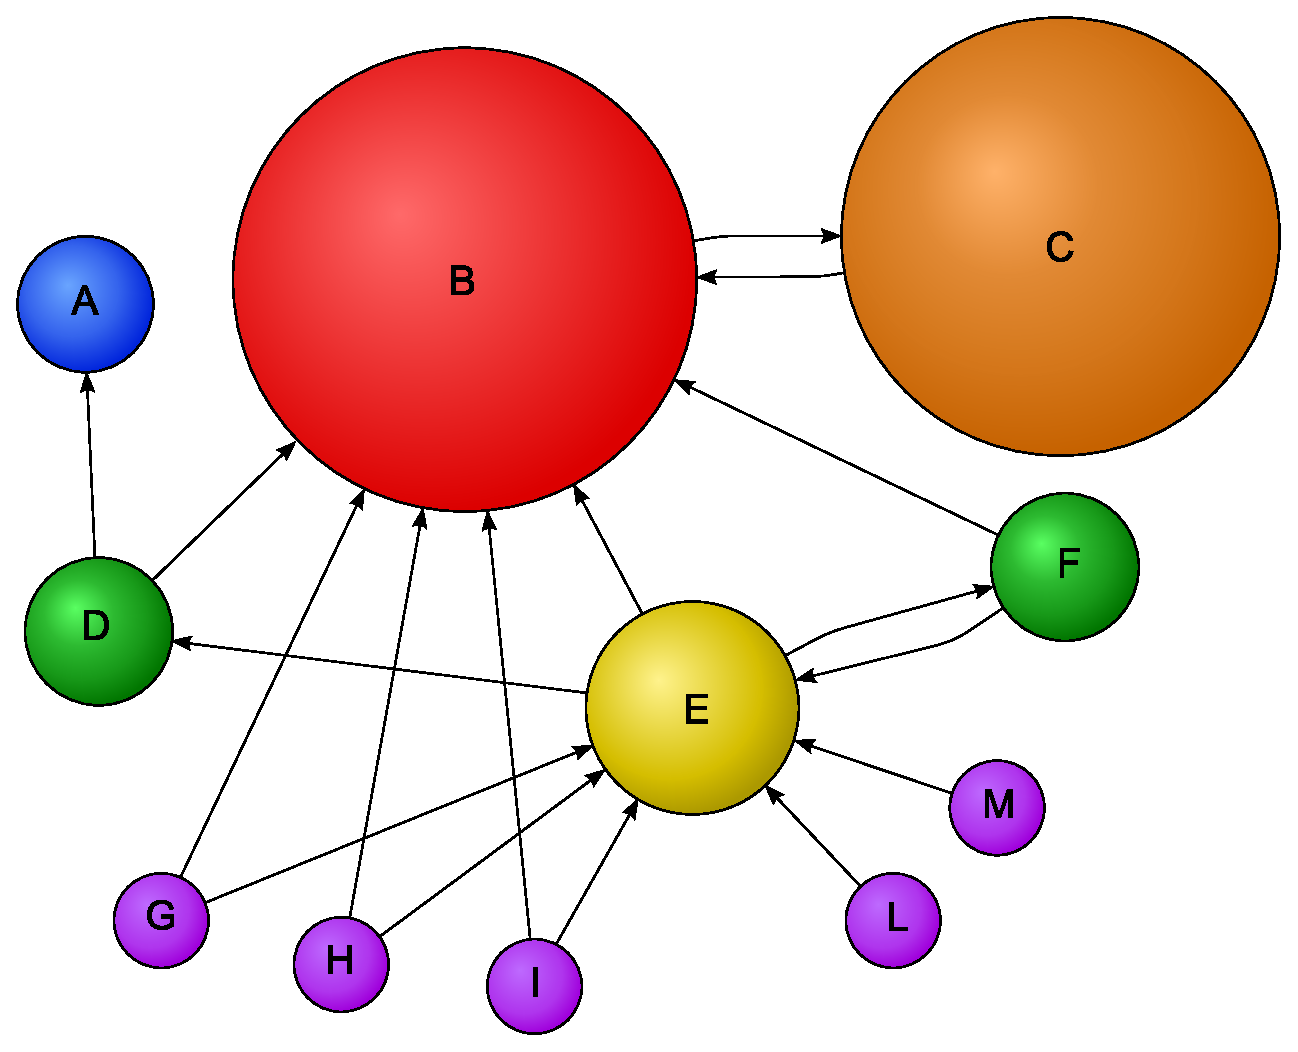
\includegraphics[width=0.6\textwidth]{./fig/PageRanks_Example_only_letters}
    \caption{Diagramma schematico del \emph{ranking}: ogni sfera rappresenta una pagina
            web, ogni freccia un link, la dimensione delle sfere \`e l'importanza
            attribuita alla pagina.}\label{fig:PR}
\end{figure}


Questo principio \`e descritto schematicamente in Fig.~\ref{fig:PR}.
La pagina B riceve molti link e quindi \`e considerata molto importante. La pagina
C \`e considerata pi\`u importante di E, anche se riceve meno link, perch\`e il voto di
B conta molto di pi\`u dei tanti ``piccoli'' voti che riceve E
(ad es. se il ``Washington Post'' o il ``New York Times'' pubblicassero un link al sito
web di ``Programmazione Avanzata per il Calcolo Scientifico'' questo varrebbe
molto di pi\`u dei link dai siti web personali di docente, esercitatore e studenti del corso!).

Dal punto di vista formale, si definisce il \emph{ranking} (importanza relativa) $r(p)$
della pagina $p$ come la somma di tutti i \emph{ranking} $r(q)$ di tutte le
pagine $q$ che puntano $p$:
\begin{align}
    \label{eq:rank}
    r(p)=\sum_{q \rightarrow p} \frac{r(q)}{\#q};
\end{align}
la somma \`e ponderata da $\#q$, numero di link presenti nella pagina $q$
(se una pagina $q$ ha un solo link verso $p$ \`e probabile che un lettore interessato lo segua,
viceversa se la pagina $q$ ha moltissimi link \`e poco probabile che il lettore scelga
proprio quello verso $p$).
\`E facile notare che si tratta di un problema in forma implicita: per conoscere il ranking di
$p$ si devono conoscere quelli delle altre pagine, che a loro volta si basano su quello di $p$.

Fortunatamente il problema \`e affrontabile in modo relativamente semplice, una volta scritto
in forma matriciale. Siano $\{p_1, p_2, \dots p_N\}$ tutte le pagine web censite e sia
$A \in \mathbb{R}^{N \times N}$ la matrice di connessione, il cui elemento $a_{i,j}$ \`e dato da:
\begin{align}
      \label{eq:harmonicp}
      a_{i,j}=
      \begin{cases}
        \dfrac{1}{\#p_j} &\qquad \mbox{se esiste un link da $p_j$ a $p_i$} \\[5mm]
        0 & \qquad \mbox{altrimenti.}
      \end{cases}
\end{align}

Si noti che gli $a_{i,j}$ possono essere intepretati come una distribuzione di probabilit\`a,
in particolare rappresentano la probabilit\`a che un persona che clicca a caso giunga alla
pagina $p_i$ a partire dalla pagina $p_j$. La matrice gode della propriet\`a:
\begin{align} \label{eq:sum1}
    \sum_{i=1}^{N} a_{i,j}=1.
\end{align}

Se il \emph{ranking} delle pagine web $p_i$ \`e rappresentato dal vettore colonn
\emph{PageRank} $\vv{r}=[r_1,r2, \dots r_n]^T$, allora l'equazione \eqref{eq:rank}
equivale al seguente problema:
\begin{align*}
    \vv{r}=A \vv{r}.
\end{align*}
Il \emph{PageRank} \`e quindi l'autovettore corrispondente all'autovalore 1 del problema
agli autovalori associato. Si pu\`o dimostrare che se i $\lambda_i$ sono gli autovalori
di $A$ allora $|\lambda_i| \leq 1$. Inoltre $\lambda_1=1$ ha molteplicit\`a
uno\footnote{Una condizione sufficiente \`e fornita dal teorema di Perron Frobenius,
che richiede una matrice corrispondente ad un grafo irriducibile. Un trucco per
soddisfare l'ipotesi potrebbe essere quello di attribuire un link ad ogni pagina
esistente alle pagine senza link.}.

Dato che il numero di pagine censite $N$ \`e dell'ordine di grandezza delle decine di
miliardi, il calcolo con un metodo diretto dell'autovettore \emph{PageRank} \`e
computazionalmente troppo oneroso, anche per chi dispone di risorse di calcolo eccezionali.
Si utilizza quindi un metodo iterativo, che restituisce una soluzione approssimata,
ad esempio ci si potrebbe basare sul metodo delle potenze. In questo caso particolare,
arrestare il numero di iterazioni al passo $k$ significa aver considerato solo le pagine
$p_j$ che distano da $p_i$ al pi\`u $k$ click\footnote{Per ragioni di semplicit\`a di
esposizione tralasciamo la possibilt\`a di introdurre un fattore di rilassamento
(\emph{damping fatctor}) \cite{Brin1998}, che comunque non modifica il principio base
dell'algoritmo.}.

\subsection*{Metodo delle potenze}

Il \emph{metodo delle potenze} \`e applicabile a matrici in cui
l'autovalore di modulo massimo $\lambda_1$ abbia molteplicit\`a
unitaria e sia ben separato dall'autovalore immediatamente pi\`u
piccolo in modulo. Il generico passo dell'algoritmo \`e riportato di
seguito:
\begin{align*}
    {\bf q}\iter{k} &= \frac{ A{\bf q}\iter{k-1} }{
        \norm{ A{\bf q}\iter{k-1}}_2 },\\
    {\bf \nu}\iter{k} &= {{\bf q}\iter{k}}^T  A {\bf q}\iter{k},\\
    {\bf w}\iter{k} &= \frac{ {{\bf w}\iter{k-1}}^T A }{
        \norm{ {{\bf w}\iter{k-1}}^T A}_2 },
\end{align*}
dove con $\nu\iter{k}$, ${\bf q}\iter{k}$ e ${\bf w}\iter{k}$ si sono
indicate, rispettivamente, le approssimazioni di $\lambda_1$ e degli
autovalori destro e sinistro ${\bf x}_1$ e ${\bf y}_1$ ad esso
associati. Vale la seguente stima, utile per determinare un criterio
d'arresto:
\begin{align*}
    \module{ \lambda_1 - \nu\iter{k} } \approx %
    \frac{ \norm{ {\bf r}\iter{k} }_2 }{
    \module{ {{\bf w}\iter{k}}^T \cdot{\bf q}\iter{k} } },
\end{align*}
dove ${\bf r}\iter{k} \eqbydef A{\bf q}\iter{k} - \nu\iter{k}{\bf
q}\iter{k}$ \`e il residuo all'iterazione $k$-esima.

\subsection*{Linear algebra library: Eigen}

In order to solve the eigenvalue problem we need a linear algebra library. In
this course we adopt the \texttt{Eigen} library version 3.1, that can manage
dense and sparse matrices.


\section*{Esercizio 1}

Starting from the example \texttt{QuadratureRule/baseVersion}
\begin{enumerate}
  \item extend the use of GetPot in order to pass the integrand function
  directly from the data file

  \item add a Gaussian quadrature rule, templatized on the number of quadrature
  points. The Gaussian rule should derive from the common base class
  \cpp{StandardQuadratureRule}. The points and weights can be computed using the
  \texttt{legendre\_rule} library

  \item compute the integral of the function
    \begin{align*}
    f(x) = e^x x
    \end{align*}
  in $[0,1]$ using all the available quadrature rules.

  \item implement a MonteCarlo quadrature rule, that also derives from
  \cpp{QuadratureRule}.
\end{enumerate}


% \section*{Solutions}

\begin{enumerate}

    \item In order to make the code reusable, we choose to group all the
    interfaces for the classes in a header file, while the implementations are
    in a corresponding source file. There is also a separate header file for
    the common definitions, such as \cpp{enum}s and \cpp{typedef}s

    \lstset{basicstyle=\scriptsize\sf}
    \lstinputlisting{./src/1/src/rootfinding.hpp}
    \lstset{basicstyle=\sf}

    In this case, the name defined by \cpp{rootfinding.hpp} are exported in the
    \cpp{Rootfinding} \cpp{namespace}.

    here follow the listings for the header file and source file that implement
    the \cpp{Bisection} and \cpp{Newton} classes.
    % Bisection
    \lstset{basicstyle=\scriptsize\sf}
    \lstinputlisting[caption=\cpp{Bisection} class interface]
      {src/1/src/bisection.hpp}
    \lstset{basicstyle=\sf}
    note that all the private attributes in the class are in the form
    \cpp{M_attributename}. This is a common approach to clearly state in the
    implementations which variables are local and which are class variables.

    The \cpp{converged} method is an \cpp{inline} function. The \cpp{inline}
    directive tells the compiler that it should try to insert the whole body of
    the function where it is called, instead of issueing a call. As it is done
    in the code, it is still possible to separate the declaration and the
    definition of the method. All the methods that are directly declared inside
    a class are treated as \cpp{inline}. If the method is instead implemented
    outside the class, it must be in a header file. It is common practice to
    insert only very short methods directly inside the class. The \cpp{inline}
    directive is available also for free functions, and it behaves in the same
    way.
    \lstset{basicstyle=\scriptsize\sf}
    \lstinputlisting[caption=\cpp{Bisection} class implementation]
    {src/1/src/bisection.cpp}
    \lstset{basicstyle=\sf}
    Inside the constructor of the class it is possible to call explicitly the
    constructors of the attributes of the class. In this case, the members 
    \cpp{M_tol}, \cpp{M_maxit} and \cpp{M_check} are initialized directly from
    the values of \cpp{tol}, \cpp{maxit} and \cpp{check}, respectively.

    The notes for the \cpp{Newton} class are analogous to the ones for the
    \cpp{Bisection} class. Here follows the listings for this class
    % Newton
    \lstset{basicstyle=\scriptsize\sf}
    \lstinputlisting[caption=\cpp{Newton} class interface]
    {src/1/src/newton.hpp}
    \lstinputlisting[caption=\cpp{Newton} class implementation]
    {src/1/src/newton.cpp}
    \lstset{basicstyle=\sf}


    \item Here follows the listings for the \cpp{Robust} class, subdivided in a
    header file and a source file.
    % Robust
    \lstset{basicstyle=\scriptsize\sf}
    \lstinputlisting[caption=\cpp{Robust} class interface]
        {src/1/src/robust.hpp}
    \lstinputlisting[caption=\cpp{Robust} class implementation]
        {src/1/src/robust.cpp}
    \lstset{basicstyle=\sf}

    inside the \cpp{Robust} class there are the definitions for the types for
    the coarse approximation of the zero (\cpp{coarseT}) and for the high order
    method used to refine the result (\cpp{fineT}). This can be useful if we
    decide to change one of the two methods with another one that uses the same
    interface. The student can try to implement as an homework a modified
    Newton method and introduce it in \cpp{Robust}. In the future we will see
    how to generalize this technique with the introduction of templates.
    The tolerance required for the coarse method is defined as the product of
    the final tolerance times the \cpp{M\_cfratio} (\emph{coarse-to-fine ratio})
    coefficient. The accessor member functions allow the access to
    non-modifiable memebers with a \cpp{const} method.

    The \cpp{Makefile} that compiles \cpp{bisection}, \cpp{newton} and
    \cpp{robust} produces a static library named \cpp{librootfinding.a}. Once
    the library is available, it can be used by other programs, such as the ones
    for \emph{Point 3}, specifying to the compiler the place (with
    \texttt{-Llib}) and the library name (with \texttt{-lrootfinding}).

    The structure for the \cpp{bisection}, \cpp{newton} and \cpp{robust} has a
    lot of common features. Replicating similar definitions is not only poor
    design, but can also lead to errors, for example if the classes must have a
    consistent interface. A better approach would be to create
    \cpp{IterativeMethod} base class from which all the other three derive.

    \item Here follows the code for the \emph{main program} for the solution of
    the third point. The implementation that it refers to is the one introduced
    in the previous points.
    \lstset{basicstyle=\scriptsize\sf}
    \lstinputlisting{./src/1/bn.hpp}
    \lstset{basicstyle=\sf}
    in this case the \cpp{Bisection}, \cpp{Newton} and \cpp{Robust} classes are
    stored in the \verb!./src/! folder.
    \lstset{basicstyle=\scriptsize\sf}
    \lstinputlisting{./src/1/bn.cpp}
    \lstset{basicstyle=\sf}

    Note in the \verb1main1 the use of two namespaces, \cpp{std} and
    \cpp{RootFinding}.

    \item Here follows the implementation for the \cpp{Robust} class. The
    overloading of \cpp{operator<<} is totally similar for the other two
    classes.
    \lstset{basicstyle=\scriptsize\sf}
    \lstinputlisting[linerange={15-29}]{./src/2/src/robust.cpp}
    \lstset{basicstyle=\sf}

    Note that the function that overloads the stream operator uses the private
    members of the class. This is the reason why it is declared as a
    \cpp{friend} function with the definition
    \lstset{basicstyle=\scriptsize\sf}
    \lstinputlisting[linerange=46-47]{./src/1.5/src/robust.hpp}
    \lstset{basicstyle=\sf}

    The code can be tested with the following \emph{main program}
    %
    \lstset{basicstyle=\scriptsize\sf}
    \lstinputlisting{./src/1.5/bn.cpp}
    \lstset{basicstyle=\sf}
    %
    and this is the corresponding \emph{output}
    \begin{verbatim}
0.707107
* Robust Method *
Tolerance           :   1e-06
Max # of iterations :   100
Convergence check   :   increment
# of iterations (C) :   3
# of iterations (F) :   4
C-to-F tol ratio    :   200000
    \end{verbatim}

\end{enumerate}


\bibliographystyle{siam}
%\bibliography{../common/bibliography}

\begin{thebibliography}{9}

\bibitem{Brin1998} S.~Brin and L.~Page,
``The anatomy of a large-scale hypertextual web search engine'',
{\em Computer Networks and ISDN Systems}, vol.~30, no.~1-7, pp.~107 -- 117,
1998. Proceedings of the Seventh International World Wide Web Conference.

\end{thebibliography}

\end{document}
